\documentclass[a4paper]{report}

\usepackage[T1]{fontenc}
\usepackage[utf8]{inputenc}
\usepackage[italian]{babel}
\usepackage{amsmath}
\usepackage{amssymb}
\usepackage{caption}
\usepackage{graphicx}
\usepackage{booktabs}
\usepackage{textcomp}


\begin{document}
\chapter{Supervised Learning e Metodi Statistici}

\section{Introduzione al Supervised Learning}
La scienza delle predizioni, o data learning, gioca un ruolo chiave in diversi campi scientifici come ad esempio quello della statistica e dell'intelligenza artificiale, grazie a procedure applicative legate principalmente al cosiddetto data mining.

In un tipico scenario di apprendimento supervisionato è presente un valore di \textit{outcome}, generalmente quantitativo (come ad esempio una quotazione finanziaria) o categorico (come ad esempio una discriminante situazionale del tipo infarto/non infarto), che si vuole predire in base ad un set \textit{features} (ad esempio dati clinici).
Avendo a disposizione un \textit{training set} di dati, dei quali è possibile osservare outcome e features per un insieme di oggetti (ad esempio una popolazione), è dunque opportuno costruire un modello predittivo, o \textit{learner}, il quale permetterà di valutare l'outcome per oggetti ignoti.

Una situazione di questo tipo è detta di \textit{Supervised Learning} in quanto è la presenza della variabile di outcome a guidare l'intero processo di apprendimento.
Introducendo un linguaggio più vicino al \textit{machine learning}, è possibile schematizzare il problema nel seguente semplice modo: si ha a che fare con un set di variabili in \textit{input}, generalmente misurate o note a priori, le quali influenzano uno o più \textit{outputs}; l'obiettivo è l'utilizzo degli input per la previsione dei valori in output.

\section{Interpolazioni Lineari e Metodi di Maximum Likelihood}
Tra i metodi più ampiamente utilizzati per la costruzione di \textit{learners} troviamo quelli che appartengono alla macrocategoria della Maximum Likelyhoood, ossia che tendono a massimizzare la cosiddetta funzione di verosimiglianza, definita in base alla probabilità di osservare una data realizzazione campionaria dipendentemente ai valori assunti dai parametri statistici oggetto di stima.

La potenza e la popolarità dei metodi appartenenti alla suddetta classe è dovuta alla relativa semplicità analitica e ad una buona stabilità nella realizzazione delle soluzioni predittive.
Due ottimi esempi di ciò sono i metodi di \textit{K-nearest Neighbor Prediction} e di \textit{Interpolazione Lineare per Minimi Quadrati (Least Squares)}; il primo fornisce soluzioni precise a partire da assunzioni strutturali poco stringenti, dunque in generale meno stabili (\textit{High Variance, Low Bias}).
Il secondo presuppone assunzioni strutturali più consistenti, il che conduce ad una stabilità maggiore nei risultati a scapito di una minore precisione (\textit{Low Variance, High Bias)}.

Per gli scopi del processo utilizzato nella produzione dei risultati relativi a questo lavoro, è opportuna una trattazione analitica più dettagliata di quest'ultimo metodo.

\subsection{Modelli Lineari e Minimi Quadrati}
Il modello lineare è uno dei capisaldi delle analisi statistiche ed anche in ambito di machine learning costituisce un potente strumento d'indagine.
Si giustificherà infatti in questa sezione il fatto che sia possibile ottenere risultati adeguati e facilmente interpretabili anche avendo a disposizione piccoli datasets o in presenza di un basso rapporto segnale-rumore, rendendo dunque il modello lineare altamente performante in termini di capacità predittiva anche in confronto a modelli più analiticamente complessi.

Dato un vettore di inputs  $X^T = (X_1,X_2,...,X_n)$, intendiamo predire l'output $Y$ attraverso il modello \[\hat{Y}=\hat{\beta_0}+\sum_{j=1}^{n}X_j\hat{\beta_j}\] dove il termine $\hat{\beta_0}$ è l'intercetta o \textit{bias} in termini di machine learning.
Al fine di creare una notazione più compatta possiamo includere la variabile costante $1$ in $X$ e $\hat{\beta_0}$ in $\hat{\beta}$, vettore dei coefficienti associati. Avremo ora la seguente formulazione per il modello \[\hat{Y}=X^T\hat{\beta}\] dove $X^T$ denota il vettore o la matrice trasposta (essendo $X$ un vettore colonna).

Nell'occorrenza in cui l'output sia unico $Y$ sarà uno scalare; in generale può però consistere di un vettore \textit{K-dimensionale}, nel qual caso $\beta$ assumerebbe la forma di una matrice di coefficienti a dimensione $n\times K$.

Vedendola come funzione nello spazio \textit{n-dimensionale} degli input $f(X)=X^T\beta$ è lineare ed il gradiente $f'(X)=\beta$ è un vettore dello spazio degli input con direzione e verso concordi con la direzione di massima pendenza.

Per il fitting del modello lineare su un training set di dati, verrà analizzato il metodo detto dei \textit{minimi quadrati}.
Questo approccio ha come obiettivo quello di trovare i coefficienti $\beta$ che minimizzano la \textit{somma quadratica dei residui}, definita da \[RSS(\beta)=\sum_{j=1}^{N}(y_i-x_i^T\beta)^2\]

La funzione $RSS(\beta)$ è una funzione quadratica dei parametri; essa ammette sempre dunque un minimo, ma non è scontata l'unicità di quest'ultimo.
Utilizzando un'agevole notazione matriciale per caratterizzare la soluzione abbiamo
\[RSS(\beta)=(\textbf{y}-\textbf{X}\beta)^T(\textbf{y}-\textbf{X}\beta)\]
dove \textbf{X} è una matrice $N \times n$ le cui righe sono vettori di input e \textbf{y} è un vettore \textit{N-dimensionale} di outputs nel training set.

Differenziando per $\beta$ si ottiene l'\textit{equazione normale}
\[\textbf{X}^T(\textbf{y}-\textbf{X}\beta)=0\]
nell'ipotesi in cui $\textbf{X}^T\textbf{X}$ sia non singolare, la soluzione unica è data da
\[\hat{\beta}=(\textbf{X}^T\textbf{X})^{-1}\textbf{X}^T\textbf{y}\]
il valore interpolato per l'\textit{i}esimo punto di input $x_i$ sarà dunque $\hat{y}(x_i)=x_i^T\hat{\beta}$. Per un arbitrario punto $x_0$ avremo dunque una previsione data da $\hat{y}(x_0)=x_0^T\hat{\beta}$.

Nel caso ad esempio in cui la funzione interpolante desiderata debba essere una semplice retta $y=bx+a$ (regressione lineare) vanno determinati univocamente i parametri $a$ e $b$ in modo da soddisfare il problema di minimizzazione generale, che si riduce alla minimizzazione della distanza euclidea tra le due successioni,$y_i$ e $f(x_i)$ data da 
\[ S = \sum_{i=1}^n \left(y_i - f(x_i)\right)^2\]

E' possibile in tal caso esplicitare i coefficienti $a$ e $b$ come
\[b=\frac{ N \sum (x_i y_i) - \sum x_i \sum y_i}{N\sum (x_i^2)-(\sum x_i)^2}\]
\[a=\frac{\sum y_i \sum (x_i^2)- \sum (x_i) \sum (x_i y_i)}{N\sum (x_i^2)-(\sum x_i)^2}\]

Le ipotesi che le osservazioni seguano una distribuzione normale, che sia cioè $x_{i}\sim N(\mu,\sigma^{2}), \forall i$, e che la grandezza $Y$ sia a queste ragionevolmente correlata come $Y=A+BX$ , fanno sì che il metodo dei minimi quadrati permetta di calcolare esattamente i parametri $\mu$ e $\sigma$ per la distribuzione, essendo questo la \textit{soluzione analitica} al problema della \textit{maximum likelihood} per una Gaussiana.

Con un ragionamento più generale, assumiamo infatti di dover cercare una correlazione qualsiasi del tipo $Y=\Phi(X)$; essa dipenderà da un certo numero di parametri in modo tale che si possa scrivere
\[Y=\Phi(X,\{\lambda_k\})\]

Per la stima dei parametri $\{\lambda_k\}$ e quindi per l'adattamento della funzione $Y=\Phi(X,\{\lambda_k\})$ ai punti sperimentali introduciamo due ipotesi di partenza:
\begin{itemize}
\item L'incertezza su $X$ è trascurabile rispetto all'incertezza su $Y$
\item L'incertezza su $Y$ è espressa in termini dello scarto quadratico medio di una distribuzione normale, cioè $\delta y_i=\sigma_i$
\end{itemize}

Se i parametri $\{\lambda_k\}$ della funzione $Y=\Phi(x,\{\lambda_k\})$ fossero noti, una volta fissato un valore $x_i$ della variabile indipendente $X$, la densità di probabilità di misurare un valore $y_i$ sarebbe
\[
f(y_i)=\frac{1}{\sigma_i \sqrt{2\pi}} exp\{- \frac{[y_i - \phi(x,\{\lambda_k\})]^2}{2\sigma_i^2}\}
\]

Fissato un insieme di $N$ valori $x_1,..,x_N$ di $X$, la densità di probabilità di ottenere una $N-pla$ di valori $y_1,...,y_N$ tra loro indipendenti è data da una densità multivariata fattorizzabile nel prodotto delle singole densità $f(y_i)$
\[
g(y_1,...,y_N;\{\lambda_k\})=\prod^{N}_{i=1}\frac{1}{\sigma_i \sqrt{2\pi}} exp\{- \frac{[y_i - \phi(x,\{\lambda_k\})]^2}{2\sigma_i^2}\}=\]
\[
=\frac{1}{(\prod_{i}\sigma_i)(2\pi)^{N/2}} exp\{-1/2\sum^{N}_{i=1} \frac{[y_i - \phi(x,\{\lambda_k\})]^2}{\sigma_i^2}\}
\]

Nella realtà sono invece noti gli $N$ valori $y_i$, mentre sono incogniti i valori dei parametri $\{\lambda_k\}$.

Le migliori stime dei parametri si hanno ora massimizzando $g(y_1,...,y_N;\{\lambda_k\}$ rispetto ad essi, ossia minimizzando la sommatoria che compare all'esponente dell'ultimo membro dell'equazione di cui sopra. 

La sommatoria viene convenzionalmente indicata come $\chi^2$

\[
\chi^2=\sum^{N}_{i=1} \frac{[y_i - \phi(x,\{\lambda_k\})]^2}{\sigma_i^2}\}
\]

Essendo ora noti i valori $x_i$ e $y_i$ e $\sigma_i$ è chiaro che la funzione $\chi^2$ è una funzione dei soli parametri $\{\lambda_k\}$
\[
\chi^2=\chi^2(\lambda_1,...,\lambda_p)
\]
definita in uno spazio \textit{p-dimensionale}.

Per determinare i $\{\lambda_k\}$ che permettono alla funzione $\Phi(x,\{\lambda_k\})$ di adattarsi meglio ai punti sperimentali è sufficiente una minimizzazione di $\chi^2$ nello spazio \textit{p-dimensionale} dei parametri.

E' importante tenere come questo tipo di trattazione non prescinda mai dal'ipotesi di normalità

E' necessario tuttavia per lo scopo finale di questo lavoro, analizzare il comportamento della funzione di massima verosimiglianza in presenza di una distribuzione Gaussiana troncata deterministicamente, a partire dalle generalità del metodo. 
Nella prossima sezione si giustificherà il fatto che i minimi quadrati non siano più ottimali per la previsione nel caso in cui non siano soddisfatte le condizioni strutturali di normalità.

\subsection{Maximum Likelihood e Distribuzioni Normali Troncate}
L'ipotesi strutturale sulla distribuzione dei residui necessaria, per l'assunzione dei minimi quadrati come funzione di massima verosimiglianza, viene meno nel caso in cui si ha a che fare con una Gaussiana troncata.

In generale è infatti presente un campionamento $x_1,x_3,..,x_n$ di $n$ osservazioni indipendenti ed identicamente distribuite, provenienti da una distribuzione la cui \textit{funzione di densità di probabilità }  $f_0(\cdot)$ non è nota. 
E' comunque assunto che essa appartenga ad una certa famiglia di distribuzioni $ \{f(\cdot |\theta),\theta\in\Theta\} $, dove $\theta$ è un vettore di parametri per la famiglia stessa detta \textit{modello parametrico}, cosicché $f_0=f(\cdot |\theta_0)$. 
Il valore $\theta_0$ non è noto ed è il \textit{valore vero} del vettore dei parametri.
E' necessario trovare un estimatore $\hat{\theta}$ il più vicino possibile al valore $\theta_0$. 

Per utilizzare il metodo di massima verosimiglianza, si procede specificando la \textit{funzione di densità complessiva} per tutte le osservazioni.
Per un campionamento indipendente e distribuito identicamente si ha
\[ f(x_1,x_2,\ldots,x_n\mid\theta) = f(x_1|\theta)\times f(x_2|\theta) \times \cdots \times  f(x_n|\theta)\]
Considerando le osservazioni $x_1,x_3,..,x_n$ come parametri fissati della funzione, $\theta$ assumerà il ruolo di variabile arbitraria; è così possibile introdurre la \textit{funzione di verosimiglianza}
\[ \mathcal{L}(\theta\,;\,x_1,\ldots,x_n) = f(x_1,x_2,\ldots,x_n\mid\theta) = \prod_{i=1}^n f(x_i\mid\theta)\]
Da un punto di vista puramente operativo è conveniente utilizzare il logaritmo della funzione di verosimiglianza (\textit{log-likelihood})
 \[\ln\mathcal{L}(\theta\,;\,x_1,\ldots,x_n) = \sum_{i=1}^n \ln f(x_i\mid\theta)\]
e considerare il \textit{log-likelihood medio}
\[\hat\ell = \frac1n \ln\mathcal{L}\]

La notazione $\hat\ell$ non è affatto casuale: essa assimila il termine ad un estimatore, cosa che in effetti $\hat\ell$ è in quanto indice di verosimiglianza logaritmica attesa per la singola osservazione.

Il metodo di massima verosimiglianza stima dunque $\theta_0$ a partire da un valore $\theta$ che massimizza $\hat\ell(\theta,x)$.

Il metodo definisce così un \textit{Maximum-Likelihood Estimator (\textbf{MLE}) } per $\theta_0$
\[\{ \hat\theta_\mathrm{mle}\} \subseteq \{ \underset{\theta\in\Theta}{\operatorname{arg\,max}}\ \hat\ell(\theta\,;\,x_1,\ldots,x_n) \}\]
La massimizzazione della log-likelihood è equivalente a quella della likelihood vera e propria, essendo il logaritmo una funziona monotona strettamente crescente.

Per la maggior parte dei modelli, può essere trovato un MLE sotto forma di funzione esplicita dei dati osservati $x_1,x_3,..,x_n$.
Qualora non fosse possibile una trattazione analitica della soluzione di massimizzazione, si utilizzano metodi numerici di ottimizzazione per il MLE.

Il problema dello slicing deterministico dei dati che questo lavoro si propone di affrontare, rende inevitabile la trattazione della distribuzione Gaussiana troncata.

A partire dalla formulazione della sua particolare \textit{funzione di densità di probabilità} sarà possibile giustificare l'impossibilità di definire una soluzione analitica per questo tipo di distribuzioni.

Supponiamo infatti che  $X \sim N(\mu, \sigma^{2}) \!$ abbia una distribuzione normale e sia confinata nell'intervallo $ X \in (a,b), \; -\infty \leq a < b \leq \infty $. 
L'aggiunta di queste  condizioni rende la distribuzione $X$ una \textit{Gaussiana troncata} nell'intervallo
$a<X<b$.

La sua funzione di densità di probabilità $f$ per $a\leq x \leq b$ assumerà dunque la forma
\[
f(x;\mu,\sigma,a,b) = \frac{\phi(\frac{x - \mu}{\sigma})}{\Phi(\frac{b - \mu}{\sigma}) - \Phi(\frac{a - \mu}{\sigma}) }{.}\frac{1}{\sigma}
\]
ed $f=0$ al di fuori dell'intervallo.

Si ha che per $	\xi=\frac{x-\mu}{\sigma}$; ${\phi(\xi)=\frac{1}{\sqrt{2 \pi}}\exp{(-\frac{1}{2}\xi^2})} $ rappresenta la funzione di densità di probabilità della \textit{distribuzione normale standard} mentre le ${\Phi(\cdot)}$ sono le \textit{funzioni di distribuzione complessiva (cumulative distribution functions)}.

La presenza delle $\Phi(\alpha),\Phi(\beta)$ con $\alpha=\frac{a-\mu}{\sigma}, \beta=\frac{b-\mu} {\sigma}$ comporta l'impossibilità di una formulazione semplice ed analiticamente definita dei parametri di massima verosimiglianza, rendendo necessaria un'ottimizzazione numerica per l'approssimazione delle soluzioni.
Questo aspetto e la proposta di possibili metodi di soluzione sono ampiamente trattati nel paper \textit{"Regression analysis when the dependent variable is truncated normal"} di Takeshi Amemiya (\textit{Econometrica, Novembre 1976, Volume 41, Numero 6}).

Questo lavoro si propone tuttavia di correggere i metodi lineari canonici, ampiamente utilizzati dagli algoritmi di \textit{machine learning}, trattando la possibilità di stimare il \textit{bias} associato all'utilizzo di un MLE non analiticamente corretto. 

In questo modo sarà possibile ottenere previsioni e risultati verosimili mantenendo la semplicità operativa propria dell'ipotesi lineare.
A questo proposito nella sezione successiva seguirà la descrizione dei metodi legati al machine learning propriamente detto.

\subsection{Train-Test Split e Cross Validation}
Tra le procedure più elementari per un approccio di machine learning alla trattazione dei dati, vi è quello del cosiddetto \textit{train and test splitting}.

Esso consiste nella divisione casuale del del dataset in due subsets: \textit{train set} e \textit{test set}.
Il train set, come il nome suggerisce, è utilizzato per elaborare i parametri utilizzando il regressore scelto.
Questi vengono poi applicati e confrontati coi dati presenti nel train set, i quali ovviamente fungendo da dati "non visti" forniscono una stima realistica della performance predittiva del regressore utilizzato, generalmente sotto forma di $R^2$

Operativamente è possibile effettuare lo splitting utilizzando algoritmi di random sorting, fornendo le percentuali di dati da utilizzare come train e test; convenzionalmente si pone la percentuale del train al $70-80\%$ dell'intero dataset, a cui segue quella del test per sottrazione.

Questa procedura, seppur elementare, sopperisce al problema del cosiddetto \textit{overfitting}, ossia la tendenza a creare un modello analitico che interpoli molto precisamente i dati sperimentali a scapito di una scarsa capacità predittiva.

Un metodo direttamente basato sul train-test splitting è quello della \textit{Cross Validation}.
Questo è probabilmente il metodo più semplice ed ampiamente utilizzato per stimare l'errore e dunque la qualità di una predizione.

La cross-validation stima in maniera diretta l'errore atteso per l'analisi riferita al subsample (che possiamo assimilare ad un test set) che rimane esterno all'elaborazione dei parametri, definito come
\[
Err=E[L(Y,\hat{f}(X)]
\]
dunque \textit{l'errore medio generalizzato} relativo all'applicazione del metodo $\hat{f}(X)$ su un test set indipendente della distribuzione correlata di $X$ e $Y$.

Idealmente, avendo a disposizione un numero sufficientemente grande di dati, potremmo isolare quello che verrà chiamato \textit{validation set} ed utilizzarlo per valutare la performance del modello predittivo utilizzato.

Tuttavia in generale si hanno a disposizione database non molto estesi, per cui questa procedura risulterebbe approssimativa.

Per sopperire al problema, si introduce la cosiddetta \textit{K-fold cross validation}, la quale usa una parte dei dati per essere interpolati dal modello scelto e un'altra per testarne le capacità predittive.

SI introduce un splitting dei dati in $K$ parti uguali; per ogni $k-esima$ parte, utilizziamo le rimanenti $k-1$ parti per il fitting del modello e sfruttiamo questa per la stima dell'errore sulla predizione.
Per una descrizione quantitativa si introducono le funzioni seguenti.

Sia $k:\{1,2,...,N\}\longmapsto\{1,...,K\}$ una funzione di indexing che indica la partizione alla quale l'\textit{i-esima} osservazione è assegnata casualmente.

Sia $\hat{f}^{-k}(x)$ la funzione interpolata, calcolata avendo rimosso la \textit{k-esima} parte dei dati.
Allora la stima dell'errore sulla predizione data dalla cross validation sarà
\[
CV(\hat{f})=\frac{1}{N}\sum^{N}_{i=1}L(y_i,\hat{f}^{-k(i)}(x_i))
\]

Delle scelte tipiche per $K$ sono $K=5,K=10$; il caso in cui si ponga $K=N$ la procedura prende il nome di \textit{leave-one-out cross-validation} e si avrà che $k(i)=i$, cosicché per ogni \textit{i-esima} osservazione il fit sarà calcolato su tutte le altre osservazioni eccetto la \textit{i-esima}.

Dato un set di modelli $f(x,\alpha)$ indicizzati tramite il parametro di curvatura $\alpha$, si indica con $\hat{f}^{-k}(x,\alpha)$ l'$\alpha-esimo$ elaborato avendo rimosso la \textit{k-esima} parte dei dati.
Per questo set di modelli definiamo allora

\[
CV(\hat{f}(x,\alpha))=\frac{1}{N}\sum^{N}_{i=1}L(y_i,\hat{f}^{-k(i)}(x_i,\alpha))
\]

La funzione $CV(\hat{f}(x,\alpha))$ fornisce una stima della curva di errore sul test; possiamo così trovare il parametro di \textit{tuning} $\hat{\alpha}$ che la minimizza. Il modello finale scelto per il fit completo dei dati sarà così $f(x,\hat{\alpha}$.

E' interessante a questo punto commentare le capacità performative della cross validation al variare della scelta di $K$.

Per $K=N$ si otterranno stime per l'errore di predizione atteso con un bias praticamente nullo, ma a causa della probabile similitudine reciproca degli $N$ training sets potrebbero presentare un'alta varianza.

Al contrario per $K=5$ ad esempio la varianza sarà bassa, ma il bias potrebbe costituire un problema a causa della sua dipendenza dalla performance del metodo di learning che varia con le dimensioni di train e test sets.

In sintesi, se la curva di learning ha un pendenza considerevole ad una certa dimensione di train o test set, la \textit{k-fold cross-validation} con $K=10,5$ sovrastimerà l'errore sulla predizione.

Il metodo \textit{leave-one-out} ha invece in generale un basso bias ma non è esclusa la possibiità di avere una varianza considerevole.











  
  
  

  











 

\chapter{Valutazione degli effetti di troncatura deterministica per popolazioni sintetiche}

\section{Introduzione al Problema}
L'utilizzo di database spesso composti su un intervallo discreto di una data popolazione, frequentemente selezionato tramite criteri che possiamo definire "deterministici" (un intervallo di età ad esempio, o in generale un certo range di valori disponibile al momento dell'acquisizione), si contrappone all'esigenza di ottenere un modello di validità generale in termini di coefficienti delle variabili e di interazione fra esse.

Nella sezione precedente è stato inoltre dimostrato come la presenza di un troncatura renda l'utilizzo del metodo dei minimi quadrati (comunque ampiamente utilizzato per elaborazioni di questo tipo) analiticamente non valido. 
Una conseguenza inevitabile di ciò è una propagazione dell'errore anche nell'ambito di attribuzione dello score dei modelli ipotetici, poiché avremo una valutazione della bontà di previsione sotto forma di $R^2$ riferita ad un metodo il cui limite di validità è trasceso.

Non è pertanto possibile elaborare un risultato che abbia la pretesa di essere generale senza tenere conto di un'analisi quantitativa dell'effetto di slicing dei set di dati, che come è dimostrato in seguito potrà fornire una correzione applicabile al modello come stima di un bias per i coefficienti in relazione alla percentuale di dati utilizzati nell'elaborazione.

I risultati di seguito riportati si riferiscono ad interpolazioni di tipo lineare, elaborate attraverso metodi di machine learning quali cross-validation e boot-strapping (precedentemente descritti).

\section{Metodi di Elaborazione}
\subsection {Generazione delle popolazioni e Data Structures}
Le popolazioni sintetiche $x_1$,$x_2$,$x_3$ sono generate in modo da essere distribuite normalmente e la $y$ sia composta secondo la relazione \[y=x_1+0.1x_1^2+x_2x_3\]con l'aggiunta del relativo rumore statistico, anch'esso simulato normalmente.
In questo modo è possibile valutare la propagazione dell'effetto non solo per termini di primo gradoma anche per  termini di grado superiore al primo e per termini d'interazione (nel caso presente sotto forma di prodotto).

Lo script genera due popolazioni ciascuna composta da $N=10^3$ individui, che successivamente vengono scalate in base alla percentuale di taglio in analisi fornita come argomento alla funzione.

In questo modo sarà sempre possibile confrontare risultati elaborati su popolazioni della stessa grandezza, una composta da elementi selezionati casualmente e che dunque sarà semplicemente una "riduzione in scala" della popolazione iniziale, l'altra composta dagli elementi presenti entro il range percentuale del taglio.

Per quest'ultima categoria di campioni lo slicing viene infatti effettuato dallo script non in maniera stocastica, ma previo sorting del dataset secondo percentili relativi alle posizioni delle singole osservazioni nell'array, vengono eliminati dati a partire dalle estremità in base alla percentuale di slicing fornita come argomento in generazione.

Questa procedura permette di imputare le discrepanze attese relativamente al ranking di modelli ipotetici e stima dei parametri per i coefficienti unicamente al bias dovuto al troncamento deterministico del dataset.

Prima di procedere con la descrizione dei metodi analitici, è utile commentare le strutture utilizzate per manipolare i dati in input; cercando di rendere il programma il più generale possibile è stata infatti introdotta un'organizzazione di tipo Design Matrix, oggetti che descrivono la  composizione matriciale per regressioni multivariate.

Sia un modello di regressione nella forma $y=X\beta+\epsilon$ dove $X$ è la design matrix, $y$ il vettore delle osservazioni sulla variabile dipendente, $\beta$ un vettore di coefficienti associati alle $X_i$ ed $\epsilon $ il vettore dei termini di errore.
Prendendo ad esempio un modello del tipo:
\[y_i = \beta_0 + \beta_1 w_i + \beta_2 x_i + \epsilon_i \]
con 7 osservazioni dipendenti dalle variabili $w$ ed $x$, si ha in termini matriciali:

\[\begin{bmatrix}y_1 \\ y_2 \\ y_3 \\ y_4 \\ y_5 \\ y_6 \\ y_7 \end{bmatrix} =
\begin{bmatrix} 1 & w_1 & x_1  \\1 & w_2 & x_2  \\1 & w_3 & x_3  \\1 & w_4 & x_4  \\1 & w_5 & x_5  \\1 & w_6 & x_6 \\ 1& w_7  & x_7  \end{bmatrix}
\begin{bmatrix} \beta_0 \\ \beta_1 \\ \beta_2  \end{bmatrix}
+
\begin{bmatrix} \epsilon_1 \\ \epsilon_2 \\ \epsilon_3 \\ \epsilon_4 \\ \epsilon_5 \\ \epsilon_6 \\ \epsilon_7 \end{bmatrix}\]
Convenzionalmente, ed anche all'interno del programma utilizzato, la matrice delle $y$ è definita come "Outcome" e quella delle $X$ come "Predictor"; in questo modo è possibile generalizzare l'elaborazione senza dover definire funzioni specifiche in relazione al numero ed al tipo di variabili introdotte.

L'analisi è dunque strutturata in due parti specifiche per valutare l'effetto di slicing su quelli che sono aspetti essenziali per l'attribuzione della capacità predittiva di un dato metodo: il ranking di modelli ipotetici per $y$, ovviamente noto quello utilizzato per la generazione, e la precisione nella stima dei coefficienti per  le $x$.

\subsection{Effetto della troncatura nell'attribuzione dello score per modelli ipotetici}
L'algoritmo utilizzato per questo tipo di analisi prevede l'uso di tecniche di Cross Validation (nel caso specifico K-Fold Cross Validation) per il calcolo della bontà di previsione del regressore fornito,  una semplice interpolazione lineare multivariata, con il quale lo script procede ad elaborare un array contenente dei modelli ipotetici, incluso quello utilizzato per la generazione delle $y$ e che può dunque essere preso come riferimento, valutandone un $R^2$ "generalizzato" tramite una popolazione di validazione selezionata casualmente a cui vengono applicati i vari coefficienti calcolati su stratificazioni di popolazioni di Train e Test diverse per ogni iterazione, anch'esse ottenute tramite random shuffling.

In questo modo è possibile simulare l'effetto di perdita di dati sensibili a causa di criteri di selezione dei campioni o in generale l'utilizzo di un range discreto di occorrenze.

L'array dei modelli di prova contiene ipotesi riferite ai singoli termini, a tutte le loro possibili combinazioni lineari, alle possibili interazioni a coppie ed a strutture più vicine al modello di generazione e dunque contenenti termini di grado superiore al primo.
Di seguito sono riportate alcune tabelle di ranking riferite a diverse percentuali di troncatura.

\begin{table}[h!btp]
\begin{tabular}{lrrrr}
\toprule
{} &  entire &  sliced &  entire val. &  sliced val. \\
\midrule
y$\sim$x2*x3+I(x1**2)+x1 &         0.685 &         0.684 &             0.665 &             0.664 \\
y$\sim$x2*x3+x1          &         0.678 &         0.678 &             0.665 &             0.664 \\
y$\sim$x2*x3             &         0.353 &         0.347 &             0.319 &             0.319 \\
y$\sim$x2*x3+I(x1**2)    &         0.345 &         0.345 &             0.331 &             0.332 \\
y$\sim$x1 + x2           &         0.315 &         0.314 &             0.314 &             0.318 \\
y $\sim$ x1              &         0.311 &         0.312 &             0.323 &             0.322 \\
y $\sim$ x1 * x2         &         0.312 &         0.312 &             0.319 &             0.323 \\
y$\sim$x1+x2+x3          &         0.313 &         0.312 &             0.323 &             0.328 \\
y$\sim$x1+x3             &         0.310 &         0.310 &             0.314 &             0.311 \\
y$\sim$x1*x3             &         0.307 &         0.307 &             0.327 &             0.325 \\
y$\sim$x3                &        -0.009 &        -0.011 &            -0.001 &            -0.002 \\
y $\sim$ x2              &        -0.005 &        -0.011 &            -0.005 &            -0.002 \\
\bottomrule
\end{tabular}
\caption{\textit{La tabella contiene gli scores relativi alle prove per popolazioni intere e tagliate ed i corrispondenti punteggi  ottenuti su popolazioni di validazione, in questo caso la percentuale di utilizzo del database è massima.}}
\end{table}

\begin{table}[h!btp]
\begin{tabular}{lrrrr}
\toprule
{} &  entire &  sliced &  entire val. &  sliced val. \\
\midrule
y$\sim$x2*x3+I(x1**2)+x1 &         0.659 &         0.260 &             0.665 &             0.494 \\
y$\sim$x2*x3+x1          &         0.646 &         0.256 &             0.664 &             0.482 \\
y $\sim$ x1              &         0.308 &         0.134 &             0.326 &             0.209 \\
y$\sim$x1 + x2           &         0.309 &         0.131 &             0.339 &             0.213 \\
y$\sim$x1+x3             &         0.306 &         0.130 &             0.329 &             0.209 \\
y$\sim$x1*x3             &         0.299 &         0.130 &             0.335 &             0.211 \\
y $\sim$ x1 * x2         &         0.303 &         0.128 &             0.330 &             0.211 \\
y$\sim$x1+x2+x3          &         0.306 &         0.128 &             0.323 &             0.210 \\
y$\sim$x2*x3             &         0.354 &         0.048 &             0.306 &             0.186 \\
y$\sim$x2*x3+I(x1**2)    &         0.352 &         0.042 &             0.338 &             0.192 \\
y $\sim$ x2              &        -0.019 &        -0.013 &            -0.005 &            -0.003 \\
y$\sim$x3                &        -0.023 &        -0.015 &            -0.001 &            -0.001 \\
\bottomrule
\end{tabular}
\caption{\textit{La tabella contiene gli scores relativi alle prove per popolazioni intere e tagliate ed i corrispondenti punteggi  ottenuti su popolazioni di validazione, in questo caso la percentuale di utilizzo del database è del 66\%.}}
\end{table}

\begin{table}[h!btp]
\begin{tabular}{lrrrr}
\toprule
{} &  entire &  sliced &  entire val. &  sliced val. \\
\midrule
y$\sim$x2*x3+x1          &         0.495 &         0.011 &             0.658 &             0.148 \\
y$\sim$x2*x3+I(x1**2)+x1 &         0.510 &         0.005 &             0.660 &             0.146 \\
y$\sim$x1+x3             &         0.215 &        -0.031 &             0.285 &             0.049 \\
y $\sim$ x1              &         0.218 &        -0.041 &             0.319 &             0.050 \\
y$\sim$x1*x3             &         0.215 &        -0.045 &             0.330 &             0.049 \\
y$\sim$x1+x2+x3          &         0.227 &        -0.047 &             0.269 &             0.046 \\
y$\sim$x2*x3             &         0.117 &        -0.058 &             0.319 &             0.047 \\
y$\sim$x3                &        -0.131 &        -0.058 &            -0.009 &            -0.001 \\
y$\sim$x1 + x2           &         0.231 &        -0.059 &             0.310 &             0.049 \\
y $\sim$ x1 * x2         &         0.225 &        -0.070 &             0.269 &             0.046 \\
y$\sim$x2*x3+I(x1**2)    &         0.094 &        -0.076 &             0.346 &             0.047 \\
y $\sim$ x2              &        -0.094 &        -0.091 &            -0.038 &            -0.005 \\
\bottomrule
\end{tabular}
\caption{\textit{La tabella contiene gli scores relativi alle prove per popolazioni intere e tagliate ed i corrispondenti punteggi  ottenuti su popolazioni di validazione, in questo caso la percentuale di utilizzo del database è del 33\%}.}
\end{table}
Si può notare come tendenza generale che la valutazione della performance predittiva fornita dalla cross-validation in riferimento all'elaborazione sulle popolazioni troncate (indicate come \textit{sliced} sulle tabelle) sia sempre piuttosto ottimistica; questo fenomeno però non deve trarre in inganno poiché se andassimo ad analizzare l'errore sulla previsione sarebbe anch'esso sovrastimato.  
Tutto ciò causa dell'utilizzo della \textit{ten-fold cross-validation} e dell'andamento generale della \textit{ curva di learning} che come descritto nel paragrafo precedente dipende fortemente dalle dimensioni dei datasets considerati. 

Come si vede dai risultati, la classifica dei modelli in relazione alla stima del peso dei termini è in generale mantenuta anche per perdite considerevoli di dati mentre la qualità della previsione riferita alle popolazioni tagliate peggiora notevolmente; resta quindi da determinare l'andamento della stima dei coefficienti in relazione alla percentuale di utilizzo dei datasets.


\subsection{Effetto della troncatura nella stima dei coefficienti }

Per la stima del bias sui coefficienti è stato necessario valutare il rapporto fra coefficienti calcolati su popolazioni intere e coefficienti ottenuti da quelle  tagliate in corrispondenza all'aumento della percentuale di dati rimossi.

 Le funzioni utilizzate per questa sezione dell'analisi sono le stesse della precedente, con l'aggiunta di un metodo che permette di accedere ai parametri per i singoli termini del modello e di un ciclo di elaborazione statstica che consente  di utilizzare mediane e deviazioni standard per il plotting.
I grafici seguenti mostrano l'andamento dei rapporti per steps di slicing del 10\%.

\begin{figure}[hbtp]
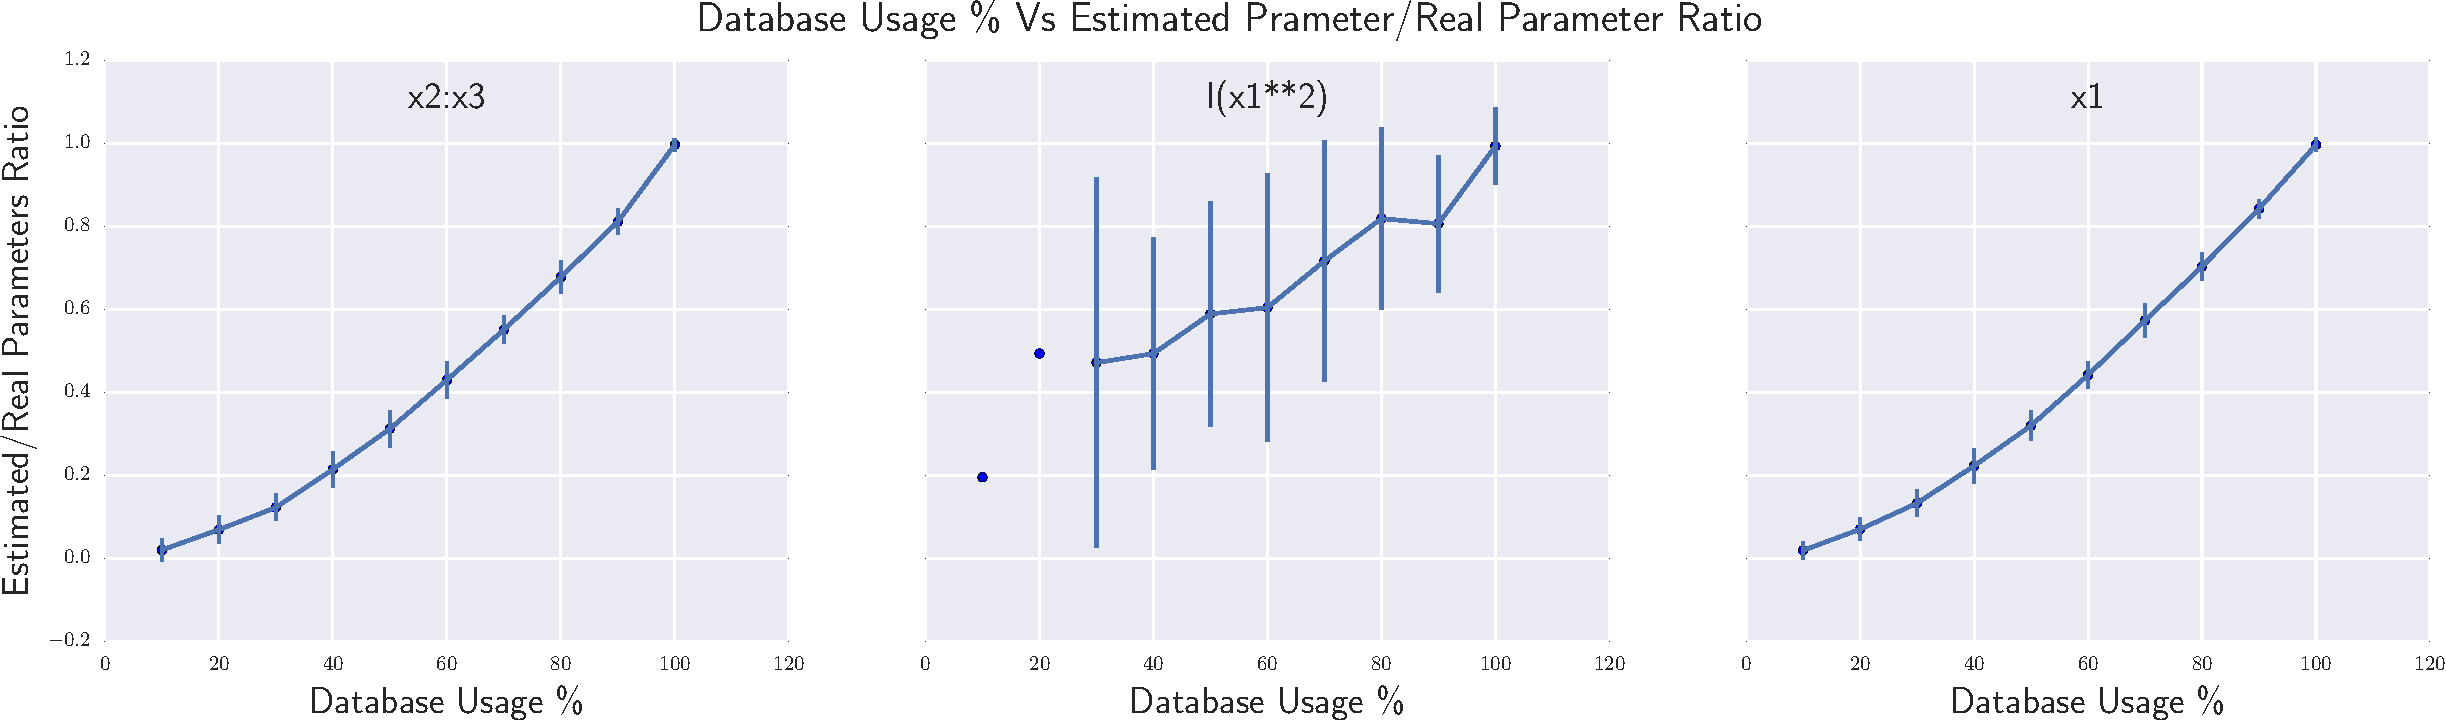
\includegraphics[width=\textwidth]{finalgraph}
\caption{\textit{Plotting della variazione del rapporto fra coefficienti in relazione al taglio del dataset. Come è evidente dal grafico al centro l'errore aumenta considerevolmente per il parametro associato al termine di grado superiore al primo a causa della sua vicinanza allo zero.}}
\end{figure}


Si può notare come l'effetto della troncatura abbia nelle migliori delle ipotesi, ossia per un'analisi fatta con dati sintetici distribuiti normalmente, un andamento lievemente esponenziale e dunque tutt'altro che trascurabile.

\chapter{Un ambiente applicativo: Il Progetto Markage}
\section{Uno sguardo al Progetto}
\subsection{Obiettivi e scopi}
Il progetto nasce in risposta al fatto che molti dei cosiddetti \textit{biomarcatori} per l'invecchiamento umano proposti dalla letteratura scientifica presentano una variabilità elevata per quanto riguarda gli studi trasversali.

Ciò implica che non sia ancora stato individuata una singola variabile che sussista da sola come marcatore utile per la determinazione dell'età biologica. Una spiegazione plausibile è data dall'intrinseca  natura \textit{multi-casuale} e \textit{multi-sistemica} dell'invecchiamento.

Lo scopo principale del progetto è quello di condurre uno studio di popolazione su circa 3200 soggetti per identificare in set di \textit{biomarcatori} per l'invecchiamento, i quali sotto forma di combinazioni di parametri a cui è attribuito un peso appropriato, siano complessivamente in grado di stimare l'età biologica in maniera più efficiente rispetto ad ogni tipo di marcatore isolato.

\subsection{Fondamenti teorici e strategie}
L'invecchiamento è stato definito come il declino dipendente dal tempo delle capacità funzionali e della resistenza agli stress, associato con il crescere del rischio di mortalità.Il processo coinvolge la maggior parte dei tessuti e degli organi del corpo.

Inoltre è da considerare la trasversalità dei processi che avvengono tra molteplici sistemi fisiologici: ad esempio l'invecchiamento del sistema metabolico 

\end{document}